\chapter{Evaluation}
\label{cha:evaluation}
 
\section{Location data characteristics for Berlin area}

\subsection{General overview}

Movement triggered data from mobile devices are spanned across the Germany as shown on \autoref{fig:ger_points}. 
\begin{figure}[!ht]
	\centering
	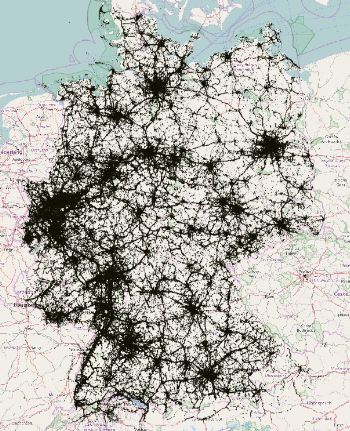
\includegraphics[width=0.3\textwidth]{images/points_germany.png}\\
	\caption{Visualisation of data points location in the geographical map of Germany}
	\label{fig:ger_points}
\end{figure}
\FloatBarrier
It points out, that most of the detected movements from one point to another are mostly gathered on the highways and inside the cities. 
\\
\begin{figure}[!ht]
	\centering
	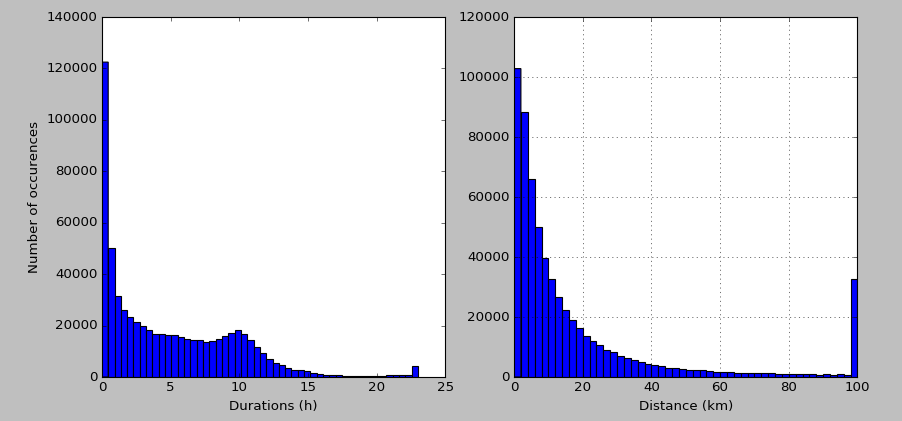
\includegraphics[width=0.9\textwidth]{images/germany_stats.png}\\
	\caption{Histograms of durations and distances between consecutive points under and cumulatively over 100 km for the area of Germany}
	\label{fig:ger_stats}
\end{figure}
\FloatBarrier
The given data batch has been gathered in the interval of 24h starting from 3am in the morning German time. It consists of over 675000 data points, belonging to 47300 unique mobile devices. \autoref{fig:ger_stats} shows, that for unique mobile devices, the durations between consecutive points in time are most frequent within 30 minutes and most of the data is in the interval 1-10h. Regarding distances, consecutive points are most frequent below 2 km and most data is in the interval 0-10km. Big chunk of distances is also over 100km.     
\\
\begin{figure}[!ht]
	\centering
	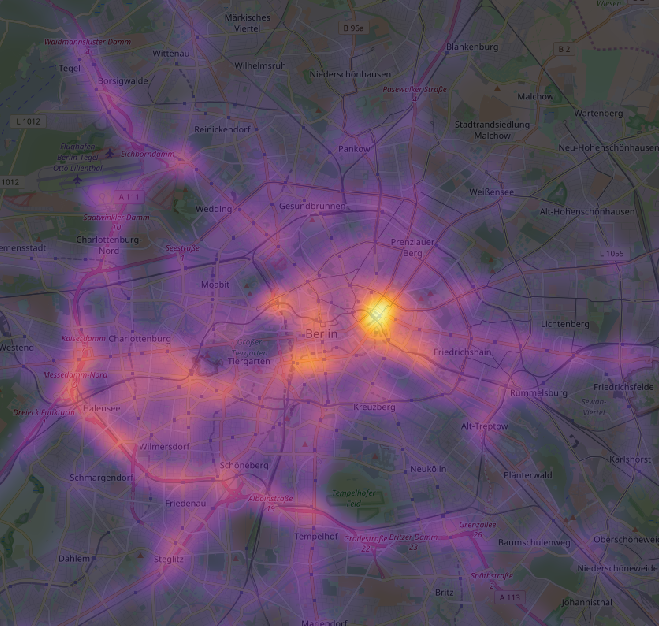
\includegraphics[width=0.9\textwidth]{images/points_berlin_heatmap.png}\\
	\caption{Heatmap of data point densities within the area of Berlin}
	\label{fig:ber_heat}
\end{figure}
\FloatBarrier
\autoref{fig:ber_heat} shows the heatmap of data points for Berlin area. We can see that most of the movements detected are on major train/tram/metro stations, highways and major living areas. 

\subsection{Data analysis}
\label{cha:dataanaly}

Statistics performed using tool written in Python (https://github.com/mrow4a/macroscopic-movements-algorithm-prototypes) shows, that for users at least once visiting Berlin, had in average 17 points gathered because of their movements in the period of 24h, harmonic mean of 4 points and maximum 100 of points.
\\
\begin{figure}[!ht]
	\centering
	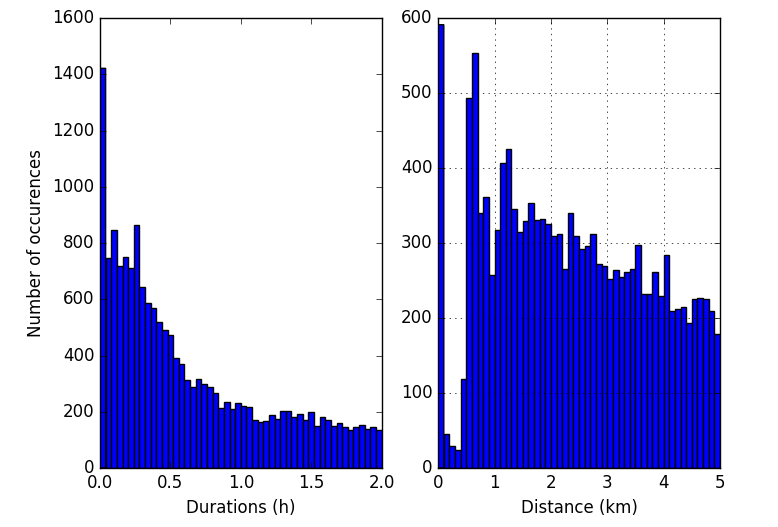
\includegraphics[width=0.6\textwidth]{images/berlin_stats_intro.png}\\
	\caption{Histograms of durations and distances between consecutive points under 5 km and under durations of 2h for the area of Berlin}
	\label{fig:ber_stats}
\end{figure}
\FloatBarrier
Furthermore, majority of durations between points is within interval of 30 minutes. For distances between points, there is significant "jump" at 500-1000m and 1100-1500m, which might mean that at these intervals, continuous points been gathered, and distances over that values might be discontinuous (ref. \autoref{fig:movement_update} ). It is due to the fact that these distance intervals are most frequent and that might suggest that this is an average "update" distance for the moving mobile devices, as described in \autoref{cha:introduction_methodo}. Less frequent values might suggest that updates were obtained with lower accuracy (e.g. by presence inside the building, metro line or simply mobile device lag in obtaining its location) and are result of discontinuity between consecutive updates.
\begin{figure}[!ht]
	\centering
	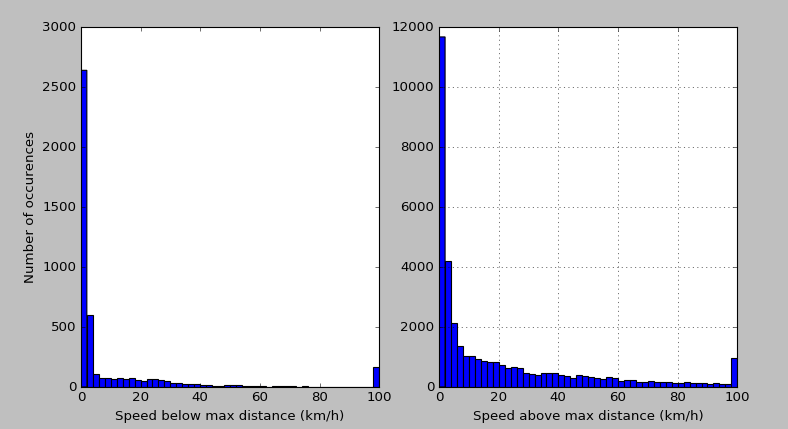
\includegraphics[width=0.6\textwidth]{images/berlin_speeds_distances.png}\\
	\caption{Histogram of speed between points with corresponding distance above or below 1.5 km}
	\label{fig:ber_sp_dis}
\end{figure}
\FloatBarrier
\autoref{fig:ber_sp_dis} shows that considering the registered distances within range of 1500m, the wast majority of points are between 0-2 km/h, and also significant interval at 2-6 km/h. The rest of the values is sparse distributed in interval 6-100+ km/h. In case of registered point above range of 1500m, we observe that indeed most frequent occurrence is at interval of 0-4 km/h, however most are sparse distributed above 4 km/h, with most points being in interval of 4-20 km/h. 

\subsection{Pre-filtering of anomalies}
\label{cha:prefilter}
\autoref{fig:ber_stats} shows that there is a fraction of points which duration or distance rapidly changed, thus resulting in very high speeds between the points. Furthermore, due to the methodology of obtaining points (movement triggered), there are some minimum distances and durations at which points can be collected, and values not matching stop or travel expectation according to gathered statistics, have to be filtered. Thus, the following predicates for filtered values have been set:
\begin{description}
	\item[Jumps] Points with speed over 83 m/s [300 km/h]
	\item[Duplicates] Points with distance below 100m and at the same time duration below 10s
\end{description}

\section{Stop Detection}

Analyzing different approaches for stop detection based on localization data (ref. \autoref{cha:introduction_appr_stopdet}), we decided to base our solution on standard human behavior regarding mobility within the cities (ref. \autoref{cha:introduction_hummob}) and reusing the concept of Mobility Index (ref. \autoref{cha:introduction_mob_index_sect})).
\\\\
Stop detection is divided into two phases:
\begin{description}
	\item[Identifying stop candidates] according to stop detection algorithm
	\item[Reconciliation of stop candidates] taking into account mobility indexes of points. 
\end{description}

\subsection{Identifying stop candidates}

Stop algorithm, shown on \autoref{fig:cd_algorithm}, is considering 3 parameters - MinWalkSpeed, MinTransportSpeed, ThresholdDistance. 
\\\\
So called ThresholdDistance is distance mentioned in \autoref{cha:introduction_dataanaly} (which in case of Berlin been in range 800-1500m) as distances between points, where there is significant "jump" in frequency of occurences, which might mean that at these intervals, continuous points been gathered, and distances over that values might be discontinuous. Furthermore, these distances are relatively small compared to other observed distances, allowing more accurate decision process. We assume, that at these distances, no significant "interuption" in gatharing the points has been introduced in the form of buildings, metro or other factors.
\\\\
Thus, for these higher accuracy points one could assume, that if mobile device have been moving within the minimum walking speed MinWalkSpeed (ref. \autoref{cha:introduction_hummob}), this point is identified as stop candidate. 
\\\\
Thus, for lower accuracy points one could assume, that if mobile device have been moving within the minimum transport speed MinTransportSpeed (ref. \autoref{cha:introduction_hummob}), this point is as well identified as stop candidate. In this example, it could mean, that over longer distance, one could move with transportation with significant speed, stop for longer period and then use fast transportation again, resulting in higher then minimum walking speed, but with speed which is in average lower then other psychological value as minimum transport speed or maximum walking speed.
\begin{figure}[!ht]
	\centering
	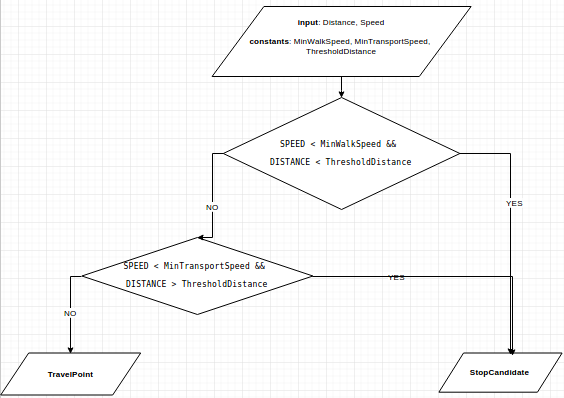
\includegraphics[width=0.8\textwidth]{images/stop_algorithm_1.png}\\
	\caption{First phase of stop detection algorithm  }
	\label{fig:cd_algorithm}
\end{figure}

\subsection{Mobility Index Analysis}

\autoref{fig:reco_general} shows that there are many scenarios in which stop candidate has been detected, taking into account movement speed between points, distance and mobility index. From the statistics about collection of points per user - \autoref{cha:introduction_dataanaly}) - the following movement profiles can be derived:
\\
\begin{description}
	\item[Standard daily movements with few relocations across the city] - In average mobile devices collected 17 points. The profile of this person could be matching e.g. - going to work in the morning, going for lunch and back, going to the shop/entertainment after work and home. This could result in points collected during transportation to those places (5-40). 
	\item[Relocations over small distances] - harmonic mean has been 4 points, which could mean that person during that day was indeed moving, but frequently requiring "area updates", thus distance covered daily was small. 
	\item[Many relocations over larger distances] - number of points collected in range above 60, might mean that user is moving a lot during the day (e.g. delivery, professional driver) or moves over long distance to another city. 
\end{description}
\begin{figure}[!ht]
	\centering
	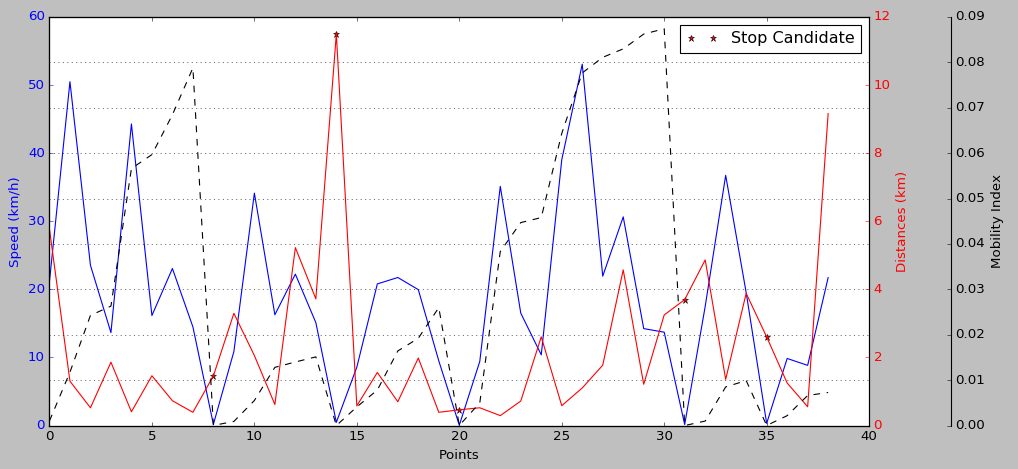
\includegraphics[width=0.8\textwidth]{images/reco_general.png}\\
	\caption{Result of identifying stop candidates for single user with their corresponding mobile index, distance and speed between the detected and previous point }
	\label{fig:reco_general}
\end{figure}
In the example for a single user over 24h shown on \autoref{fig:reco_general}, stop detection algorithm identified 5 stops. The dashed line represents the mobility index which was considering past 60 minutes from each of the points, representing how movable was that person in the last 60 minutes till that point. Analyzing mobility index in the above example (ref. \autoref{cha:introduction_mob_index_sect}), we identify "rising mobility periods" as periods of mobility/transportation, while rapid drop, as very low mobility/stay indicator.Worth notifying is that mobility index in that example very accurately correlates with the identified stop candidates. 
\begin{figure}[!ht]
	\centering
	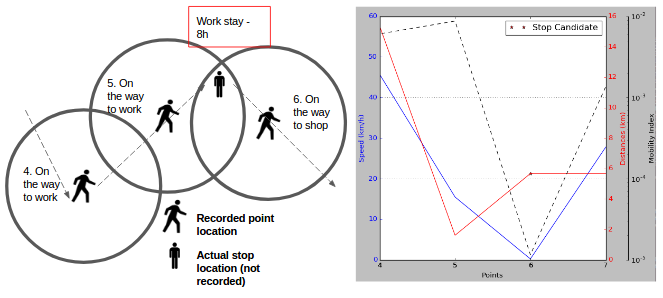
\includegraphics[width=0.9\textwidth]{images/reco_example_1.png}\\
	\caption{ Correlation of the real life example (left) to the graph of distance, speed and mobility index between consequtive points (right) }
	\label{fig:reco_ex_1}
\end{figure}
\\
Due to the method of obtaining the data - \autoref{fig:reco_ex_1} - one cannot precisely identify the location of the stop, it can be closer to Point 5, Point 6 or somewhere in the middle the two. Furthermore, statistically, most stops identified have  mobility index below certain threshold \textbf{(10e-3)} - which can be taken as a point of reference for other considerations - meaning that user continued movement, but with low speed.
\FloatBarrier

\subsection{Reconciliation of stop candidates}

\begin{figure}[!ht]
	\centering
	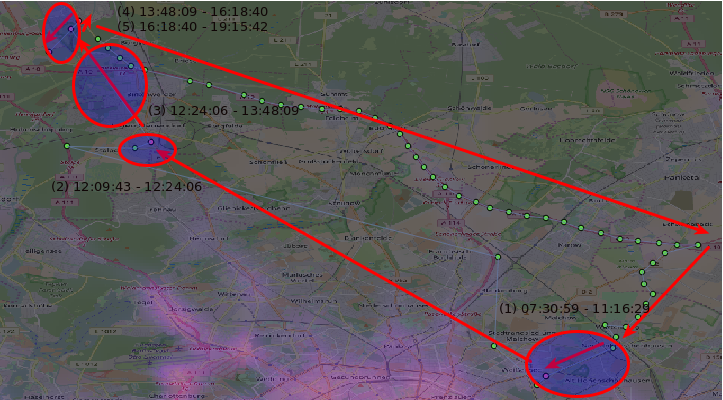
\includegraphics[width=0.6\textwidth]{images/reco_example_2b.png}
	\caption{ Movement example for one user in the period of 24h, with recorded locations due to the movement and annotated timestamps for detected stop candidates }
	\label{fig:reco_ex_2b}
\end{figure}
\begin{figure}[!ht]
	\centering
	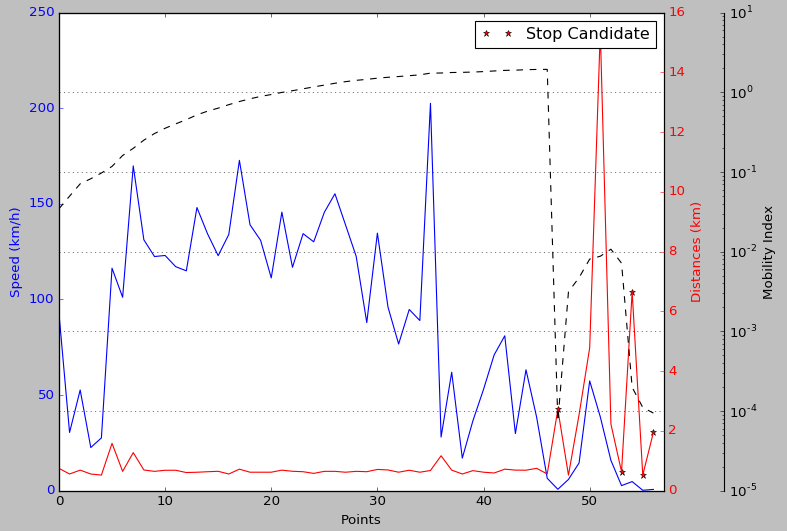
\includegraphics[width=0.6\textwidth]{images/reco_example_2a.png}
	\caption{ Visualization of distances, speed and mobility indexes for example from \autoref{fig:reco_ex_2b} with identified stop candidates }
	\label{fig:reco_ex_2a}
\end{figure} 
Analyzing traces from \autoref{fig:reco_ex_2b} and \autoref{fig:reco_ex_2a}, we identify that user has been moving from Point 0 to Point 47, in the time period 06:59 - 07:30. In between Point 47 and Point 48, the stop candidate has been identified. We notice, that from Points 0-47, measurement has been continuously gathered over a distance. This could mean, that user stopped somewhere around Point 47, stayed there some time, and when he left that location, after around 3 km from that point, at 11:16 user has been recorded in location Point 48, starting his journey to Point 54. Thus, Stop Candidate at Point 48 is meaning in that case Stop might be close to Point 47 on that way (previous to stop candidate). 
\\\\
At Point 54, we recorded Stop Candidate, however, considering that its mobility index being high (above 10e-3, also validated by small distance and walking speed covered between 12:09-12:24) and next mobility index being low, we can assume that this Stop Candidate is not a stop and have to be ignored, it is most likely approaching to the stop location. 
\\\\
In between Points 54-55, we record another Stop Candidate, in period from 12:24-13:48 and over significant distance. Recorded mobility index is low, and because it is over long distance, we assume that Stop is close to Point 54 on the way to Point 55. 
\\\\
Due to the small distance covered in between Points 55-56 and Points 56-57, we expect that the Stop Points in that cases are somewhere in between or around these Points. 
\begin{figure}[!ht]
	\centering
	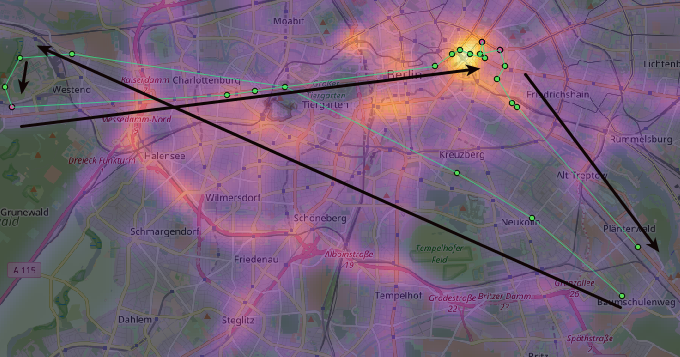
\includegraphics[width=0.6\textwidth]{images/reco_example_5a.png}
	\caption{ Visualization of distances, speed and mobility indexes for example from \autoref{fig:reco_ex_5b} with identified stop candidates }
	\label{fig:reco_ex_5a}
\end{figure} 
\begin{figure}[!ht]
	\centering
	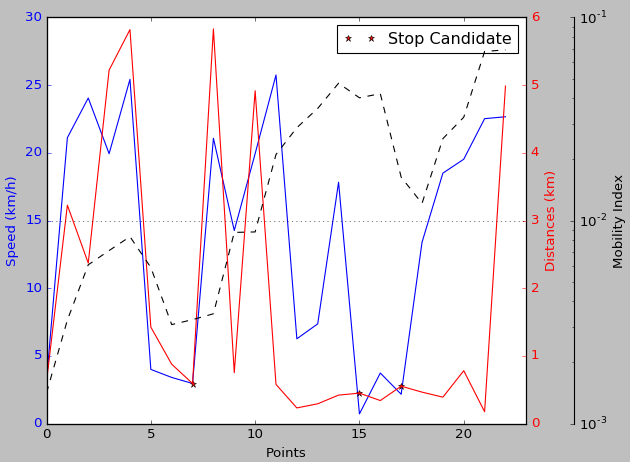
\includegraphics[width=0.6\textwidth]{images/reco_example_5b.png}
	\caption{ Movement example for one user in the period of 24h, with recorded locations due to the movement and annotated timestamps for detected stop candidates }
	\label{fig:reco_ex_5b}
\end{figure}
\\
Analyzing traces from \autoref{fig:reco_ex_5b} and \autoref{fig:reco_ex_5a} we identify example in which person is constantly moving between 8:28-12:04, and having 3 short stops in range 15-40 minutes, in Points 7, 15, 17. Mobility index in both examples is above the mobility index threshold, however, in the next point that person is again moving (above mobility index threshold), which might identify short stay at that location. 
\\\\
Further examples, showing the above mentioned events can be found in \autoref{appendix:add_example_1}, \autoref{appendix:add_example_2}
\\\\
\textbf{TODO: Now should decide what should be algorithm based on above mentioned values, most probably for:
\\-> mobility index higher then the threshold, and next point mobility index being lower then the threshold, there is no stop, but slow movement to possible stop location. 
\\-> mobility index higher then the threshold, and next point mobility index being also higher then the threshold might mean that there is short stop at the location
\\-> short distance covered, stop is either in both current and previous or in between
\\-> for long distance the stop is close to previous point}

\section{Clustering algorithm}

In this section we will describe how we evaluated our dbscan algorithm and the choice of the \textit{epsilon} and \textit{minimum points per cluster} parameter.

\subsection{DBSCAN}

We visualised our results in QGIS, a powerful graph visualisation tool. Running the dbscan with different parameters resulted in different cluster sizes and number of clusters. We started off with the target area of Berlin. The \textit{epsilon} parameter (radius of the cluster) was chosen by looking at the graininess (accuracy) of our given data set. The accuracy between points was 110 meters, this distance is refered to as \textit{accuracy distance}.
We took Alexanderplatz in Berlin as an example cluster (a popular train stop area in Berlin). We interpret one cluster as being one stop point of interest, and for this application want Alexanderplatz to be represented as one cluster. Setting the \textit{epsilon} parameter to the \textit{accuracy distance},  110 meters, gave us good looking clusters whilst higher value of the parameter resulted in clusters being unnaturally large and distance below the \textit{accuracy distance} resulted in only single-point clusters (points are stacked at the same location). Note that the \textit{minPts}, minimum points per cluster, parameter is not taken into \textit{consideration} here (it is set arbitary and only determines the number of clusters, while we here are interested in the \textit{size} of the clusters). See figures below.

\begin{figure}[!ht]
	\centering
	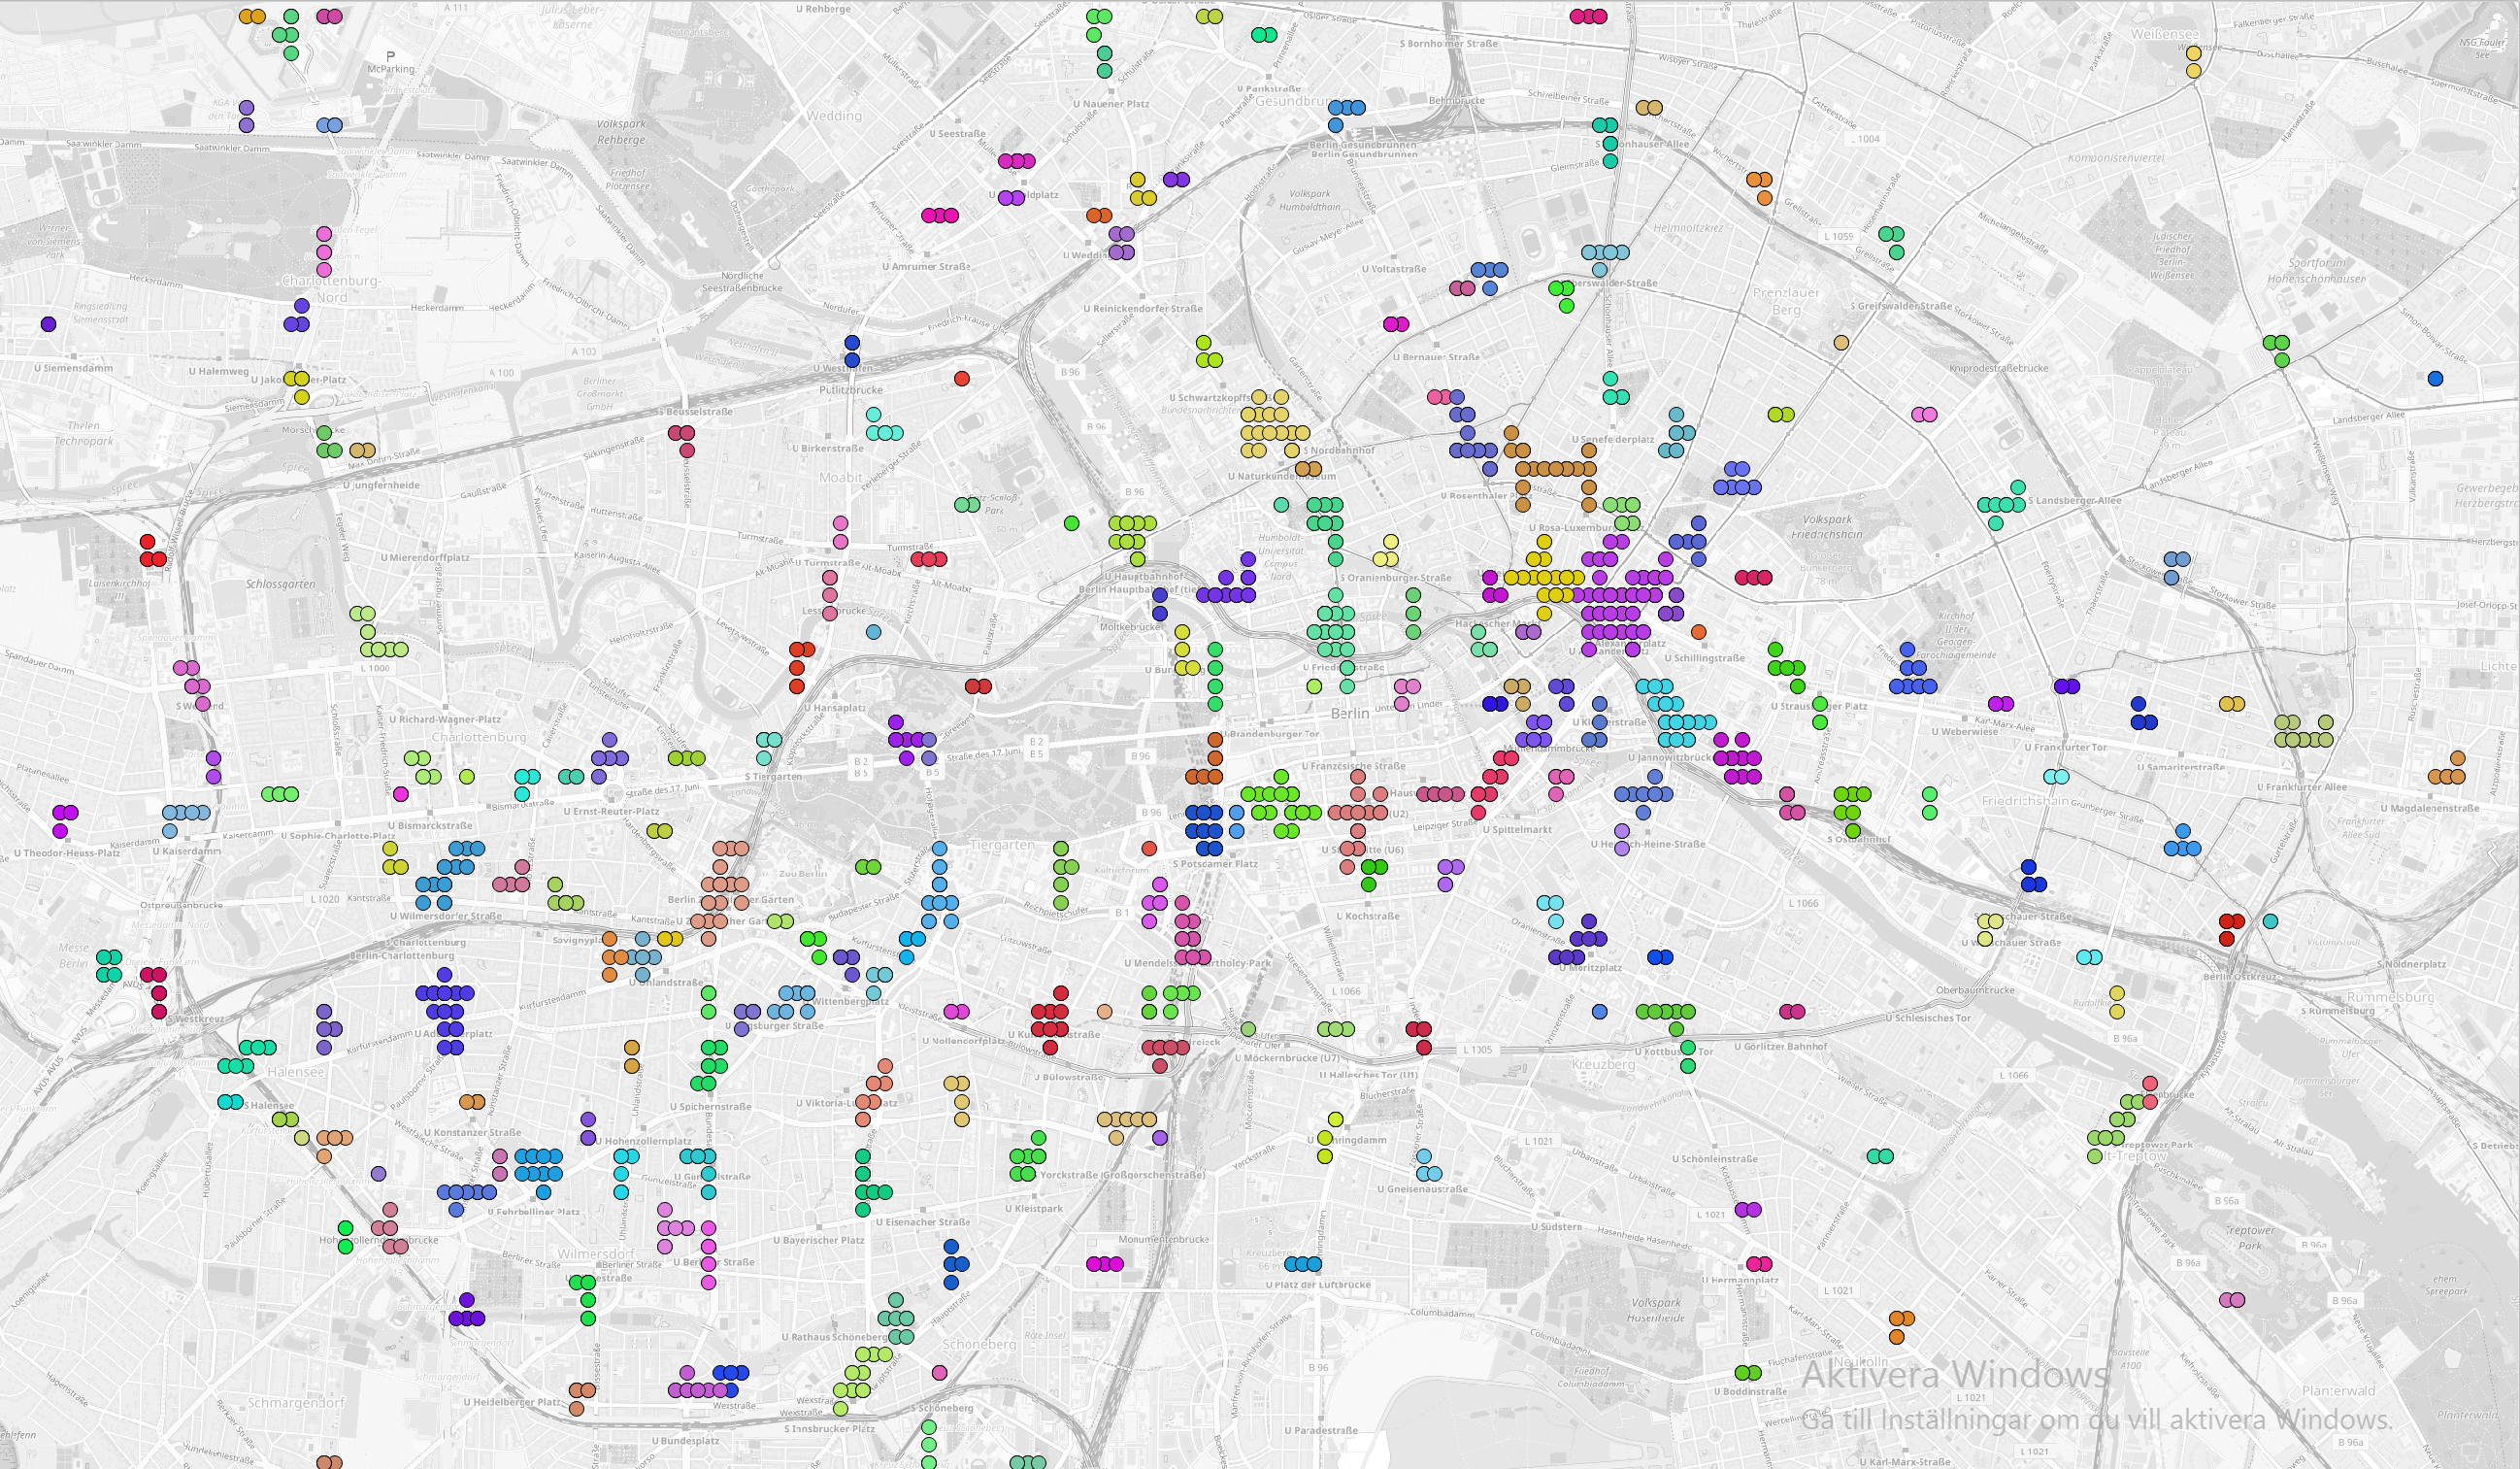
\includegraphics[width=1\textwidth]{images/0,001_5_gray.png}\\
	\caption{ Clusters with good parameters \textit{epsilon} = 110 meter, \textit{minPts} = 5. Alexanderplatz (pink) has 85 data points in it.  }
	\label{fig:0.001_5_gray}
\end{figure}

\begin{figure}[!ht]
	\centering
	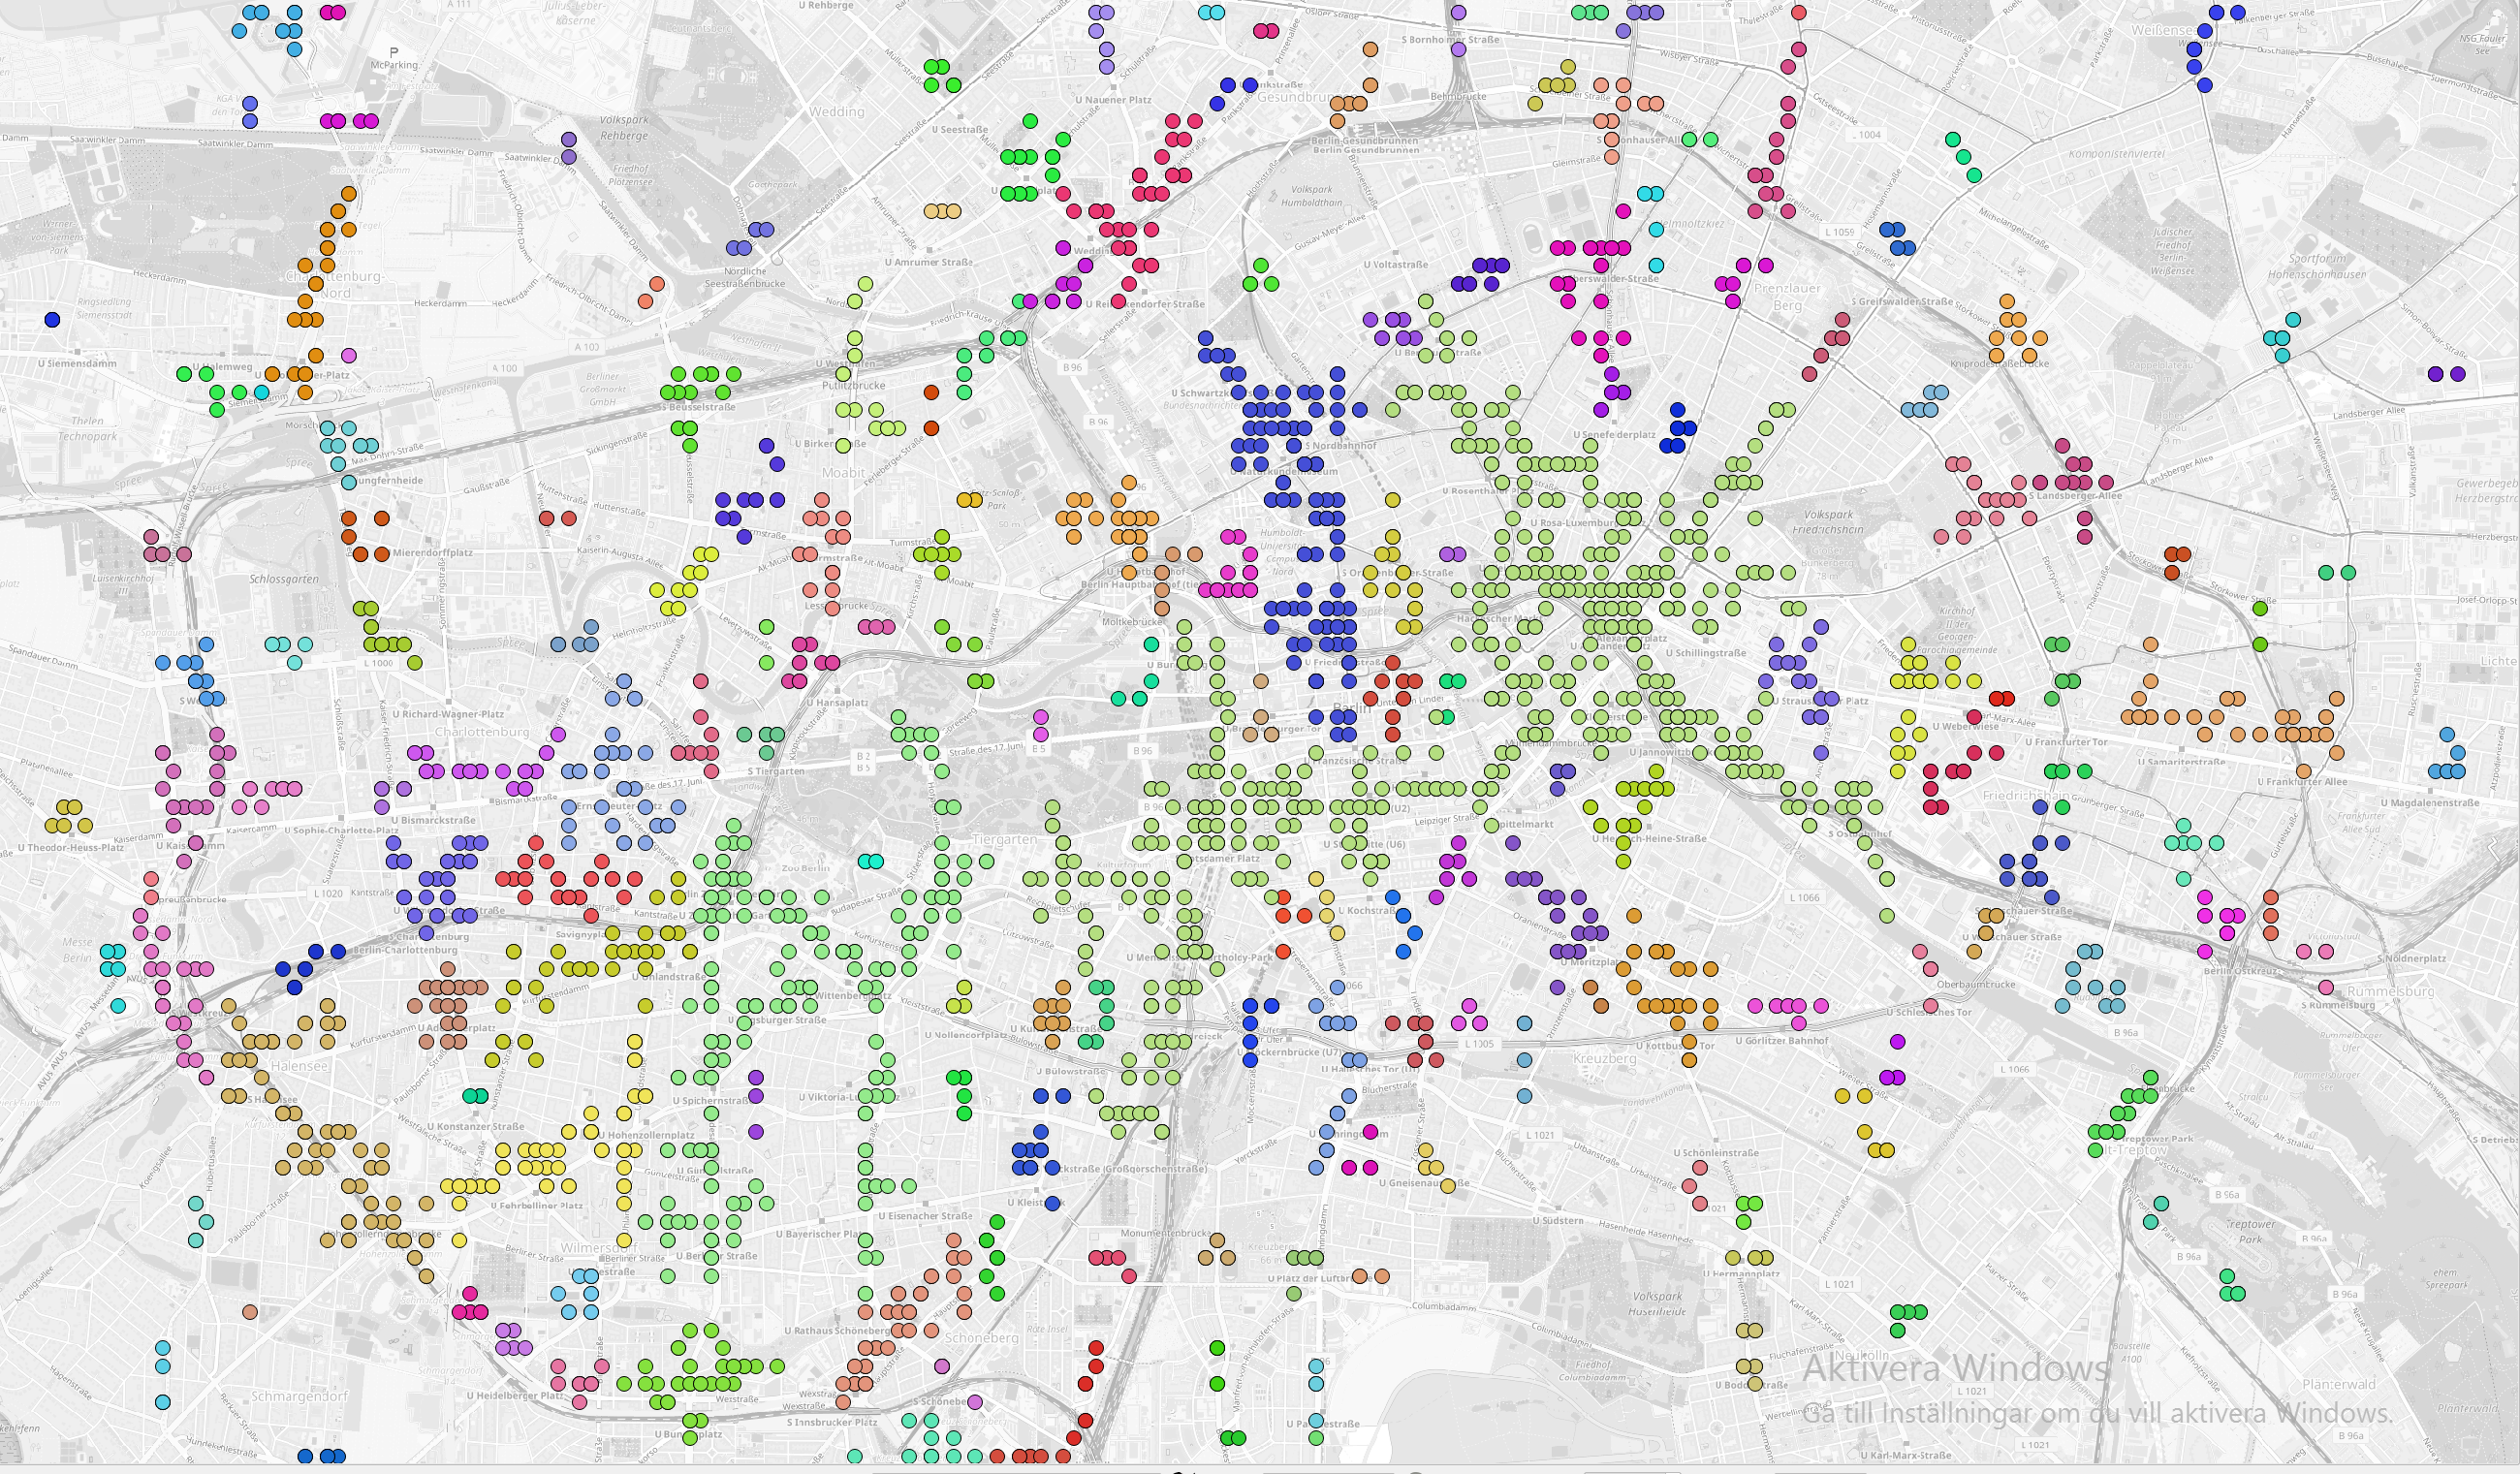
\includegraphics[width=1\textwidth]{images/0,002_5_gray.png}\\
	\caption{ Example of a clusters with bad parameters, here \textit{epsilon} = 220 meter is too large, \textit{minPts} = 5. "Alexanderplatz" (light green) has 748 data points in it and stretches over the whole centre (Mitte) of Berlin. }
	\label{fig:002_5_gray}
\end{figure}